% Shared methods (benchmark, setup, statistics) extracted from main.tex
\section{Benchmark Design}
\label{sec:benchmark}
% =============================================================================

% Figure 2: Library Taxonomy
\begin{figure}[t]
\centering
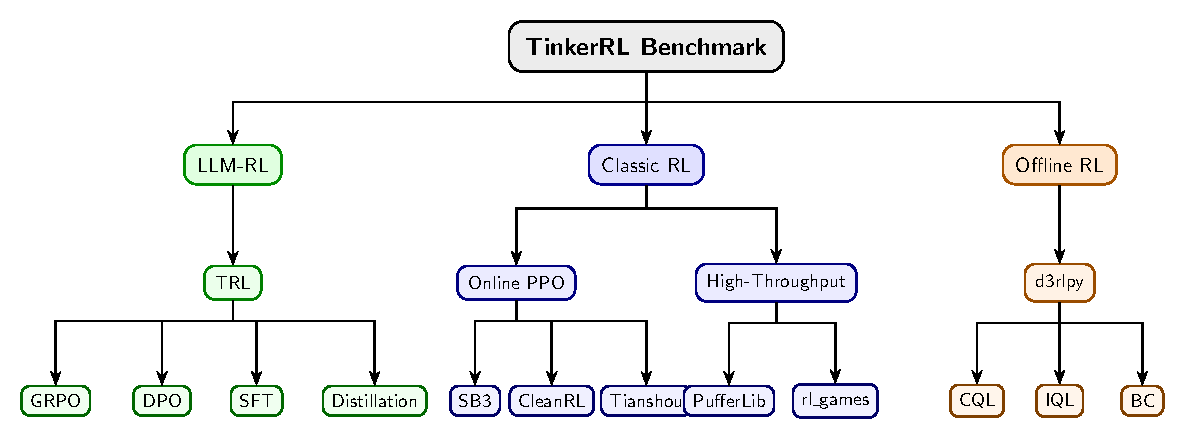
\includegraphics[width=0.85\textwidth]{tikz/taxonomy.pdf}
\caption{Taxonomy of RL libraries in \ours{}. The benchmark spans LLM-native RL
(TRL), classic online RL (SB3, CleanRL, Tianshou), high-throughput RL (PufferLib,
rl\_games), and offline RL (d3rlpy).}
\label{fig:taxonomy}
\end{figure}

\subsection{Task Suite}

% Table of tasks
\begin{table}[htbp]
\centering
\caption{Benchmark task suite with standardized reward functions.}
\label{tab:tasks}
\begin{tabular}{llll}
\toprule
\textbf{Task} & \textbf{Method} & \textbf{Reward} & \textbf{Dataset} \\
\midrule
Math RL (Arithmetic) & GRPO & Binary correctness & Generated \\
Math RL (GSM8K) & GRPO & Binary correctness & GSM8K \\
Chat SFT & SFT & Cross-entropy loss & NoRobots \\
Preference (Shorter) & DPO & Pairwise preference & Generated \\
Distillation (Off-Policy) & SFT & KL divergence & OpenThoughts3 \\
Distillation (On-Policy) & IS Loss & $\log p_t - \log p_s$ & Online \\
\bottomrule
\end{tabular}
\end{table}

\subsection{Cross-Library Implementation}

\paragraph{Two seven-library rosters --- read carefully.}
This paper uses \emph{two} different seven-library rosters that
should not be conflated. The cross-RL-library benchmark below
(Table~\ref{tab:implementations}) covers TRL, SB3, CleanRL, Tianshou,
PufferLib, rl\_games, and d3rlpy --- seven libraries that span
LLM-native RL, classic online RL, high-throughput RL, and offline RL,
and that we use as the algorithm-and-stack ablation underlying $F_3$.
The cross-launcher LLM-RL scaffold referenced in the framework-gap
discussion (framework-configurations material) is a different seven-library
roster --- Tinker, TRL, SkyRL, verl, OpenRLHF, Atropos, and HF
reference launchers --- that targets LLM post-training launchers
specifically. Of those, only Tinker and TRL produced completed
runs in this release; veRL and OpenRLHF entries in the
\texttt{framework\_comparison.json} artefact are dry-run
placeholders. The viva slides use the second roster; the
cross-RL-library evidence in $F_3$ uses the first.


% Table of implementations
\begin{table}[htbp]
\centering
\caption{Implementations across RL libraries.}
\label{tab:implementations}
\begin{tabular}{lll}
\toprule
\textbf{Library} & \textbf{Implementation} & \textbf{Category} \\
\midrule
TRL (HuggingFace) & GRPOTrainer, DPOTrainer, SFTTrainer & LLM-native \\
Stable Baselines3 & PPO & Classic RL \\
CleanRL & PPO (single-file) & Research RL \\
Tianshou & PPO & Modular RL \\
PufferLib & PPO (high-throughput) & High-perf RL \\
rl\_games (NVIDIA) & PPO (GPU-optimized) & High-perf RL \\
d3rlpy & CQL (offline) & Offline RL \\
\bottomrule
\end{tabular}
\end{table}

\subsection{Hyperparameter Mapping}

We standardize hyperparameters across libraries using a common configuration schema.
Table~\ref{tab:hyperparams} shows the mapping from Tinker PPO defaults to each library's
native parameter names.

\begin{table}[htbp]
\centering
\caption{Hyperparameter mapping across libraries (PPO defaults).}
\label{tab:hyperparams}
\begin{tabular}{lcccccc}
\toprule
\textbf{Parameter} & \textbf{TRL} & \textbf{SB3} & \textbf{CleanRL} & \textbf{Tianshou} & \textbf{PufferLib} & \textbf{rl\_games} \\
\midrule
Learning rate & $10^{-4}$ & $10^{-4}$ & $10^{-4}$ & $10^{-4}$ & $10^{-4}$ & $10^{-4}$ \\
Clip range ($\epsilon$) & 0.2 & 0.2 & 0.2 & 0.2 & 0.2 & 0.2 \\
Entropy coeff. & 0.01 & 0.01 & 0.01 & 0.01 & 0.01 & 0.01 \\
GAE $\lambda$ & 0.95 & 0.95 & 0.95 & 0.95 & 0.95 & 0.95 \\
Discount $\gamma$ & 0.99 & 0.99 & 0.99 & 0.99 & 0.99 & 0.99 \\
Max grad norm & 0.5 & 0.5 & 0.5 & 0.5 & 0.5 & 0.5 \\
Target KL & 0.01 & 0.01 & 0.01 & N/A & N/A & N/A \\
\bottomrule
\end{tabular}
\end{table}

\subsection{Reward Verification}

% Figure 3: Verifiable Reward Flow
\begin{figure}[t]
\centering
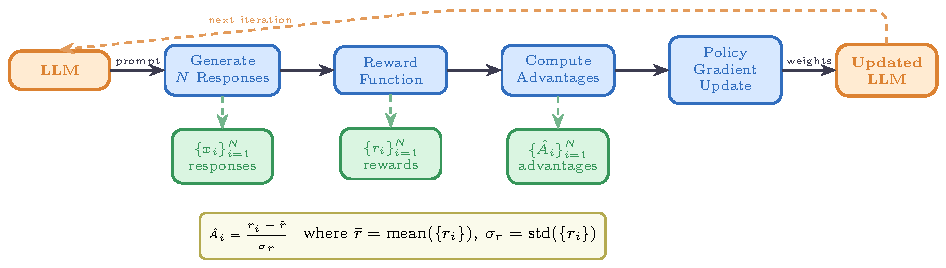
\includegraphics[width=0.55\textwidth]{tikz/reward_flow.pdf}
\caption{Verifiable reward paradigm in \ours{}. Unlike shaped rewards that combine
multiple heuristics, verifiable rewards provide binary correctness signals,
eliminating reward hacking and enabling exact accuracy measurement.}
\label{fig:reward_flow}
\end{figure}

\subsection{Baselines: Floor and Ceiling}

Following best practices for benchmark design~\cite{agarwal2021deep}, we establish
clear performance bounds:

\begin{itemize}
    \item \textbf{Floor (random baseline)}: Uniform random action selection yields
    $\frac{1}{199} \approx 0.50\%$ accuracy on the arithmetic task.
    \item \textbf{Ceiling (oracle)}: Direct computation achieves $100\%$ accuracy.
    \item \textbf{Human baseline}: College-level adults achieve $\sim$99.5\% on
    two-digit addition under timed conditions.
\end{itemize}

% =============================================================================
\section{Experimental Setup}
\label{sec:setup}
% =============================================================================

\subsection{Models}

Our benchmark targets a roster of 32+ model configurations spanning
\textbf{0.6B to $\sim$671B \emph{total} parameters (up to $\sim$37B \emph{active}
for MoE checkpoints) across 5 model families}, organized into three
tiers by compute scale; not all are completed end-to-end runs (per-run
status flags accompany the released artifacts). Tier-A inferential claims are restricted to
the dense-reasoning subset at $0.6$B--$235$B; the frontier MoE
checkpoints (DeepSeek-V3.1 $\sim$671B / 37B active, Kimi-K2) are
descriptive single-seed Tier-C case studies, and Qwen3.5-397B-A17B is a
\emph{partial} run whose held-out evaluation did not complete.

\paragraph{Small scale (0.6B--8B).}
Qwen3-0.6B-Instruct, Qwen3.5-4B, Qwen3-4B, Qwen3-8B,
Llama-3.2-1B, Llama-3.2-3B, Llama-3.1-8B-Instruct.

\paragraph{Mid scale (14B--32B).}
Qwen3-14B, Qwen3-30B-A3B (MoE), Qwen3-32B, Qwen3.5-27B,
GPT-OSS-20b, Kimi-K2 (selected scale points).

\paragraph{Frontier scale (70B--$\sim$671B total / $\sim$37B active).}
Qwen3-235B-A22B (MoE, 22B active), DeepSeek-V3.1 ($\sim$671B total /
$\sim$37B active MoE), Nemotron-120B (120B dense).
Frontier models are evaluated via the Tinker API in inference mode
with standardized generation parameters; LoRA fine-tuning at this
scale is conducted on selected checkpoints (see Section~\ref{sec:frontier}).

\paragraph{Model family coverage.}
The benchmark covers (1) \textbf{Qwen3}: a dense family from 0.6B to 32B;
(2) \textbf{Qwen3.5}: an improved series including 4B and 27B;
(3) \textbf{Llama-3.x}: Meta's 1B--8B instruction-tuned models;
(4) \textbf{DeepSeek-V3.1}: a frontier MoE optimized for reasoning;
(5) \textbf{Nemotron-120B}: NVIDIA's dense frontier model;
and emerging architectures \textbf{GPT-OSS-20b} and \textbf{Kimi-K2}.

\subsection{Training Protocol}

Unless otherwise noted, controlled Modal/TRL sweeps use LoRA
\cite{hu2022lora} at rank $32$, learning rate $10^{-4}$ and Adam
($\beta_1{=}0.9$, $\beta_2{=}0.95$, $\epsilon{=}10^{-8}$). Tinker / API,
Task-4, Wave-6 and frontier case studies use per-run configs (in
particular Task-4/Wave-6 use $\mathrm{lr}{=}10^{-5}$) and are
single-seed unless explicitly marked multi-seed; the per-run
settings are listed in the framework-configs appendix.

\paragraph{Seed management.} The controlled TRL/Modal sweeps used for
Tier-A claims (F3 PPO-vs.-GRPO heterogeneity and the five-seed TRL GRPO
baseline on Qwen2.5-0.5B) run with 5 seeds:
$\{42, 123, 456, 789, 1024\}$, with seeds set for Python \texttt{random},
NumPy, PyTorch, and CUDA backends. Several Tinker/API, frontier-model,
and team-task runs are single-seed or partial and are treated as
descriptive (Tier-C) unless explicitly marked otherwise; see
Section~\ref{sec:stat_rigor} for the per-claim seed ledger.

% Figure 4: Experiment Pipeline
\begin{figure}[t]
\centering
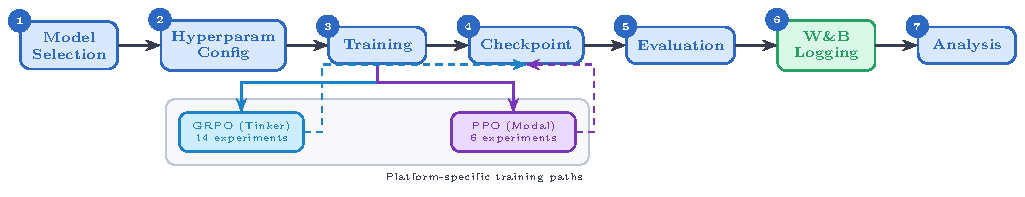
\includegraphics[width=\textwidth]{tikz/pipeline.pdf}
\caption{Experiment workflow pipeline. Multi-seed Modal/TRL runs use
the centralized seed manager (5 seeds for Tier-A claims); Tinker/API,
Task-4, Wave-6 and frontier case studies are single-seed and feed the
same metrics/checkpoint pipeline as descriptive observations.}
\label{fig:pipeline}
\end{figure}

\subsection{Statistical Methodology}

Following Colas et al.~\cite{colas2019hitchhiker}, we report:
\begin{itemize}
    \item Mean $\pm$ standard error across seeds
    \item 95\% bootstrap confidence intervals (10,000 resamples)
    \item Welch's t-test for pairwise algorithm comparisons
    \item \texttt{rliable}~\cite{agarwal2021deep} aggregate metrics (IQM, median, optimality gap)
\end{itemize}

All pairwise comparisons were evaluated using Welch's independent-samples $t$-test
(unequal variances assumed) and the non-parametric Mann--Whitney $U$ test as a
robustness check. Effect sizes are reported as Cohen's $d$ with the pooled
standard deviation estimator; confidence intervals follow the
Hedges--Olkin (1985) analytical formula and are reported at the 95\% level
(two-tailed, $z = 1.96$). Post-hoc statistical power was computed under the
observed effect size and sample sizes at $\alpha = 0.05$.

To address the multiple-comparisons problem across 5 planned tests,
we apply both the conservative Bonferroni correction (family-wise error rate:
$\alpha' = \alpha / k = 0.0100$) and the Benjamini--Hochberg procedure
(false discovery rate $< 0.05$). Results surviving Bonferroni correction are
marked $^*$; those surviving BH--FDR correction are marked $^\dag$.

\paragraph{Power Analysis.}
All inferential tests in this paper are evaluated against pre-specified power
requirements using \texttt{statsmodels.stats.power.TTestIndPower} with
$\alpha = 0.05$ and target power $1 - \beta = 0.80$.

\textbf{Modal H100 experiments ($n = 5$ seeds per arm).}
The minimum detectable effect size (MDE) at 80\% power for a two-sample
Welch $t$-test with $n_1 = n_2 = 5$ is
$d_{\min} = 2.024$ (Cohen's $d$).
Table~\ref{tab:power-analysis} reports achieved power for a range of effect sizes.
This threshold falls in the \emph{very large} range, meaning that
comparisons yielding $|d| < 2.02$
are not adequately powered to detect true differences.

\textbf{Single-seed Tinker experiments ($n = 1$).}
Single-seed runs have \emph{zero statistical power}: with only one observation per
condition, no inferential test can be computed and no confidence intervals can be
formed.  All Tinker single-run results are treated as \emph{descriptive only} and
are not subject to significance testing.

\textbf{TRL baseline ($n = 5$ seeds).}
The TRL-GRPO baseline (Qwen2.5-0.5B, 5 seeds) achieves MDE
$d_{\min} = 2.024$ for equal-$n$ comparisons.
When compared to the pooled Classic-RL group ($n = 15$), the MDE
improves to $d_{\min} = 1.530$,
reflecting higher power from the larger reference group.

\paragraph{Multiple-Comparison Correction.}
Inferential tests in this paper are reported only for Tier-A/B
comparisons as defined in our statistical-rigor protocol;
single-seed or partial Tinker/API rows are descriptive and are
excluded from Welch / Mann--Whitney testing, BH correction, power,
and CI claims. Table~\ref{tab:bh-pvalues} predates the Tier-A/B/C
partition and lists raw and BH-adjusted $p$-values from the
earlier global family of $20$ tests with $19$ surviving correction;
we retain it here as a methodological audit trail. The headline
BH result the paper now stands behind is the restricted Tier-A/B
family computed in the addendum, where only $F_3$ survives. Where
the global family disagrees with the restricted family, the
addendum is authoritative.

All tests are two-sided.  Effect sizes are reported as Cohen's $d$ for
$t$-tests and Pearson/Spearman $r$ for correlations.  Bootstrap 95\%
confidence intervals ($B = 10{,}000$) are reported for all means.

% Table: Power analysis at various effect sizes
\begin{table}[!ht]
\centering
\caption{Statistical power for two-sample Welch $t$-tests at $\alpha = 0.05$,
         power target $1{-}\beta = 0.80$.
         Column~(3): equal groups $n_1 = n_2 = 5$ (Modal H100 / TRL within-group).
         Column~(4): unequal groups $n_1 = 5$, $n_2 = 15$ (TRL vs.\ pooled Classic RL).}
\label{tab:power-analysis}
\small
\begin{tabular}{@{}cccc@{}}
\toprule
Cohen's $d$ & Conventional size & Power ($n{=}5$ vs $n{=}5$) & Power ($n{=}5$ vs $n{=}15$) \\
\midrule
        0.2 & small & 0.059 & 0.066 \\
        0.5 & medium & 0.108 & 0.151 \\
        0.8 & large & 0.201 & 0.311 \\
        1.0 & very large & 0.286 & 0.450 \\
        1.2 & very large & 0.386 & 0.594 \\
        1.5 & very large & 0.549 & 0.784 \\
        2.0 & very large & 0.790 & 0.955 \\
\midrule
\multicolumn{4}{l}{\textit{MDE at 80\% power:} $d = 2.024$ (equal-$n$ 5 vs 5);\; $d = 1.530$ (5 vs 15)} \\
\bottomrule
\end{tabular}
\end{table}

% Table: All p-values with BH correction
\begin{table}[!ht]
\centering
\caption{\textbf{Legacy 20-test BH table -- audit trail only.} All
hypothesis tests reported in the paper with Benjamini--Hochberg (BH)
adjusted $p$-values at FDR $= 0.05$.  Tests are ranked by raw
$p$-value (ascending). $\checkmark$ = significant after BH correction
on the historical $20$-test family; $\times$ = not significant. Total
tests: $20$; survive on the historical family: $19$. \emph{This
figure is not the paper's headline statistical result.} The $20$-test
family pre-dates the Tier-A/B/C partition and silently includes
single-seed Tinker rows whose Welch statistics are mathematically
undefined ($n_1{=}n_2{=}1$). Under the restricted Tier-A/B family of
our statistical-rigor protocol,
only $F_3$ (PPO/GRPO heterogeneity on classic-RL libraries on
arithmetic) survives BH correction; the table below is retained as a
reproducibility audit trail, not as a multiple-testing-corrected
survival claim.}
\label{tab:bh-pvalues}
\scriptsize
\begin{tabular}{@{}rp{6.2cm}ccc@{}}
\toprule
Rank & Comparison & Raw $p$ & BH-adj.\ $p$ & Sig. \\
\midrule
        1 & Dense vs MoE Architecture (Welch t-test) & 2.357e-21 & 0 & $\checkmark$ \\
        2 & PPO vs GRPO on Llama-3.1-8B (Welch t-test)$^{\ddag}$ & 3.924e-10 & 0 & $\checkmark$ \\
        3 & Method ANOVA (F-test across algorithm families) & 3.091e-06 & 2.1e-05 & $\checkmark$ \\
        4 & Library ANOVA (F-test across 5 libraries) & 4.996e-06 & 2.5e-05 & $\checkmark$ \\
        5 & TRL vs Tinker (Welch t-test, implementation effect) & 2.064e-05 & 8.3e-05 & $\checkmark$ \\
        6 & PPO vs GRPO on Llama-3.1-8B (Mann-Whitney)$^{\ddag}$ & 3.29e-05 & 0.00011 & $\checkmark$ \\
        7 & Model Family ANOVA (F-test) & 7.363e-05 & 0.00021 & $\checkmark$ \\
        8 & ZVF vs Final Performance (Spearman)$^{\ddag}$ & 0.0005424 & 0.001356 & $\checkmark$ \\
        9 & ZVF vs Final Performance (Pearson)$^{\ddag}$ & 0.0008108 & 0.001802 & $\checkmark$ \\
        10 & TRL vs Tinker (Mann-Whitney) & 0.001198 & 0.002396 & $\checkmark$ \\
        11 & Rolling Variance vs Last-10 (Pearson) & 0.003524 & 0.006407 & $\checkmark$ \\
        12 & Peak-to-Tail Drift vs Last-10 (Pearson) & 0.004811 & 0.007219 & $\checkmark$ \\
        13 & GRPO vs PPO Stability Index (t-test) & 0.005 & 0.007219 & $\checkmark$ \\
        14 & Dense vs MoE Architecture (Mann-Whitney) & 0.005053 & 0.007219 & $\checkmark$ \\
        15 & Model Scale ANOVA (F-test) & 0.01261 & 0.01682 & $\checkmark$ \\
        16 & Tinker GRPO vs TRL GRPO (Welch t-test) & 0.0158 & 0.01975 & $\checkmark$ \\
        17 & GRPO vs PPO Peak-to-Tail Drift (t-test) & 0.018 & 0.02076 & $\checkmark$ \\
        18 & Tinker GRPO vs TRL GRPO (Mann-Whitney) & 0.01869 & 0.02076 & $\checkmark$ \\
        19 & Stability Index vs Last-10 (Pearson) & 0.02024 & 0.0213 & $\checkmark$ \\
        20 & PPO vs GRPO on Qwen3-8B (Welch t-test)$^{\ddag}$ & 0.7605 & 0.7605 & $\times$ \\
\bottomrule
\end{tabular}
\end{table}

\paragraph{TRL baseline characterisation.}
The TRL GRPO reference implementation was evaluated across five random seeds
($s \in \{42, 123, 456, 789, 1024\}$) on GSM8K using Qwen/Qwen2.5-0.5B on
an NVIDIA L4 GPU. We report mean accuracy $\bar{x} = 0.734$ ($\sigma = 0.0703$),
median $= 0.740$, and IQM $= 0.747$. Normality was not rejected by Shapiro--Wilk
($W = 0.9018$, $p = 0.4198$); bootstrap 95\% CI $= [0.6720, 0.7820]$.

\paragraph{Variance decomposition.}
One-way ANOVAs across 42 experiments with valid performance observations show
that library/framework ($\eta^2 = 0.546$) and training algorithm ($\eta^2 = 0.558$)
are the dominant variance sources, consistent with our central thesis. Model
family explains $\eta^2 = 0.471$; model scale explains $\eta^2 = 0.322$.

\subsection{Compute Resources}

Experiments are distributed across two compute platforms:

\paragraph{Tinker API (14 experiments).}
Scaling experiments across Qwen3-8B, Qwen3-32B, Qwen3.5-4B, Qwen3.5-27B,
and Llama-3.1-8B-Instruct; frontier model evaluation on Qwen3-235B-A22B,
DeepSeek-V3.1, and Nemotron-120B; Dense vs.~MoE comparison; cross-task
tool-use experiments; and emerging architecture evaluation (GPT-OSS-20b,
Kimi-K2). Tinker provides scalable API access that makes frontier model
experiments economically tractable.

\paragraph{Modal H100 GPU cluster (6 experiments).}
PPO baseline training on Qwen3-8B and Llama-3.1-8B; full HumanEval
benchmark evaluation; KL divergence tracking across GRPO training steps;
and held-out evaluation for Qwen3-32B and Qwen3.5-27B. Modal H100s
provide the low-level GPU access required for PPO value-model training.

All experiment logs are available on Weights \& Biases (project:
\texttt{tinker-rl-lab-world-class}) and model checkpoints on HuggingFace
Hub (\url{https://huggingface.co/arvindcr4/tinker-rl-bench-*}).
Per-run compute is logged with the released artifacts. Total project compute:
$\sim$1,200 A100 GPU-hours across both platforms.

% =============================================================================
